\documentclass[dvipdfmx,cjk,10.2pt]{beamer} 
%\documentclass[dvipdfm,cjk]{beamer} %% オプションは環境や利用するプログラムに
%\documentclass[dvips,cjk]{beamer}   %% よって変える

\usepackage{subfigure}
\usepackage[all]{xy}
\usepackage{wrapfig}

\newcommand{\C}{\mathbb{C}}
\newcommand{\D}{\mathbb{D}}
\newcommand{\R}{\mathbb{R}}
\newcommand{\Q}{\mathbb{Q}}
\newcommand{\Z}{\mathbb{Z}}
\newcommand{\N}{\mathbb{N}}

\newcommand{\Imag}{\mathrm{Im}}
\newcommand{\id}{\mathrm{id}}


\makeatletter
\newcommand\xleftrightarrow[2][]{%
  \ext@arrow 9999{\longleftrightarrowfill@}{#1}{#2}}
\newcommand\longleftrightarrowfill@{%
  \arrowfill@\leftarrow\relbar\rightarrow}
\makeatother

\AtBeginDvi{\special{pdf:tounicode 90ms-RKSJ-UCS2}} %% しおりが文字化けしないように
%\AtBeginDvi{\special{pdf:tounicode EUC-UCS2}}

\setbeamertemplate{navigation symbols}{} %% 右下のアイコンを消す
\setbeamertemplate{theorems}[normal font] %%斜体を直す

\usetheme{CambridgeUS}         %% theme の選択
%\usetheme{Boadilla}           %% Beamer のディレクトリの中の
%\usetheme{Madrid}             %% beamerthemeCambridgeUS.sty を指定
%\usetheme{Antibes}            %% 色々と試してみるといいだろう
%\usetheme{Montpellier}        %% サンプルが beamer\doc に色々とある。
%\usetheme{Berkeley}
%\usetheme{Goettingen}
%\usetheme{Singapore}
%\usetheme{Szeged}

%\usecolortheme{rose}          %% colortheme を選ぶと色使いが変わる
%\usecolortheme{albatross}

%\useoutertheme{shadow}                 %% 箱に影をつける
\usefonttheme{professionalfonts}       %% 数式の文字を通常の LaTeX と同じにする

%\setbeamercovered{transparent}         %% 消えている文字をうっすらと表示する


\theoremstyle{definition}
\setbeamertemplate{theorems}[numbered]  %% 定理に番号をつける
\newtheorem{Thm}{定理}[section]
%\theoremstyle{example}
\newtheorem{Ex}[Thm]{例}
%\newtheorem{exam}[thm]{Example}
\newtheorem{Rem}[Thm]{注意}
\newtheorem{Conj}[Thm]{予想}
\newtheorem{Def}[Thm]{定義}
\newtheorem{Prob}[Thm]{問題}

\setbeamercolor{block title}{fg=blue!70!black, bg=blue!15!white} 
\setbeamercolor{block body}{fg=black, bg=blue!10!white}



\begin{document}
\title{微分・積分 第6回} 
\author{慶応義塾大学}            %% ここに書かれた情報は色々なところに使われるので
\institute[]{総合政策学部・環境情報学部}   %% なるべく設定した方が良い
\date{}



\begin{frame}                  %% \begin{frame}..\end{frame} で 1 枚のスライド
\titlepage                     %% タイトルページ
\end{frame}

%\begin{frame}                  %% 目次 (必要なければ省略)
%\tableofcontents
%\end{frame}






%%%%%%%%%%%%%%%%%%%%%%%%%%%%%%%%%%%%%%%%%%%%%%%%%%%%%%%%%%%%%%%%%%%%%%%%%%%%%%%%%%%%%%%
%%%%%%%%%%%%%%%%%%%%%%%%%%%%%%%%%%%%%%%%%%%%%%%%%%%%%%%%%%%%%%%%%%%%%%%%%%%%%%%%%%%%%%%

\section{講義概要}


\begin{frame}
\frametitle{今日の内容}



\begin{enumerate}
\item 逆写像, 逆関数, 逆関数の微分
\item 逆三角関数, 逆三角関数の微分
\end{enumerate} 



\end{frame}




%%%%%%%%%%%%%%%%%%%%%%%%%%%%%%%%%%%%%%%%%%%%%%%%%%%%%%%%%%%%%%%%%%%%%%%%%%%%%%%%%%%%%%%
%%%%%%%%%%%%%%%%%%%%%%%%%%%%%%%%%%%%%%%%%%%%%%%%%%%%%%%%%%%%%%%%%%%%%%%%%%%%%%%%%%%%%%%


%%%%%%%%%%%%%%%%%%%%%%%%%%%%%%%%%%%%%%%%%%%%%%%%%%%%%%%%%%%%%%%%%%%%%%%%%%%%%%%%%%%%%%%
%%%%%%%%%%%%%%%%%%%%%%%%%%%%%%%%%%%%%%%%%%%%%%%%%%%%%%%%%%%%%%%%%%%%%%%%%%%%%%%%%%%%%%%



\section{逆写像}


\begin{frame}
\frametitle{全射, 単射}

写像$f:X\rightarrow Y$に対して, 
$\Imag f =\{ f(x) \ | \ x \in X\} \subset Y$であった. 
\begin{Def}
\begin{enumerate}
\item $f$が\underline{全射}であるとは$\Imag f = Y$が成立すること. 
つまり「どの$y \in Y$に対しても$x \in X$が存在して$y=f(x)$」. 
\item $f$が\underline{単射}であるとは「$x_1\ne x_2$ならば$f(x_1)\ne f(x_2)$」が成立すること. 
同値な対偶条件は「$f(x_1)= f(x_2)$ならば$x_1= x_2$」.  
\item $f$が\underline{全単射}であるとは, 全射かつ単射であること. 
\end{enumerate}
\end{Def}

例: あみだくじは全単射. 

\vspace{-2mm}

 \begin{figure}[htbp]
 \begin{center} 
  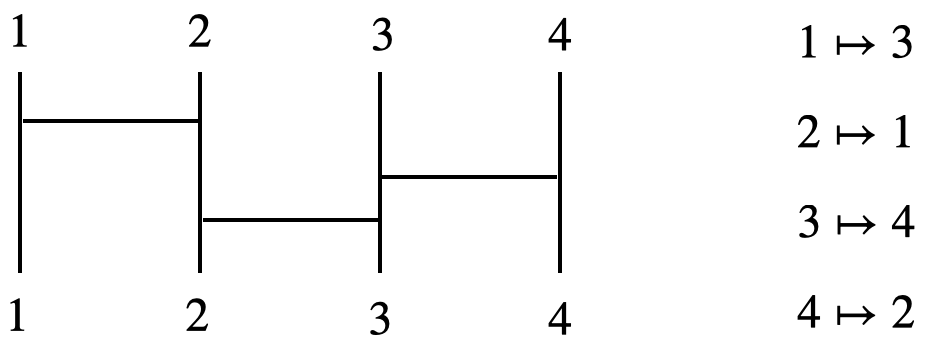
\includegraphics[width=60mm]{amida.png}
 \end{center}
\end{figure}

\vspace{-2mm}


\end{frame}

%%%%%%%%%%%%%%%%%%%%%%%%%%%%%%%%%%%%%%%%%%%%%%%%%%%%%%%%%%%%%%%%%%%%%%%%%%%%%%%%%%%%%%%
%%%%%%%%%%%%%%%%%%%%%%%%%%%%%%%%%%%%%%%%%%%%%%%%%%%%%%%%%%%%%%%%%%%%%%%%%%%%%%%%%%%%%%%



\begin{frame}
\frametitle{逆写像}


\begin{Thm}
写像$f:X\rightarrow Y$が全単射であれば, 写像$g:Y\rightarrow X$が存在して, 
$$
g\circ f = \id, \ \ \ f \circ g = \id
$$
が成立する. 
この$g$を$f$の\underline{逆写像}といい, $f^{-1}$と書く. 
\end{Thm}

実際, 任意の$y \in Y$に対して, $x \in X$で$f(x)=y$なるものが唯一つ存在するので, $g(y)=x$と定義すれば良い. 
\vspace{-4mm}

 \begin{figure}[htbp]
 \begin{center} 
  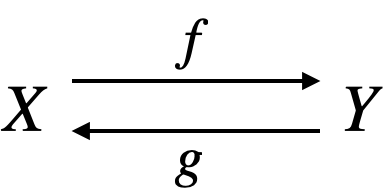
\includegraphics[width=25mm]{inverse.png}
 \end{center}
\end{figure}

\vspace{-2mm}

特に$X \subset \R$, $Y \subset \R$のときに, 逆写像を逆関数と呼ぶ. 

\end{frame}


%%%%%%%%%%%%%%%%%%%%%%%%%%%%%%%%%%%%%%%%%%%%%%%%%%%%%%%%%%%%%%%%%%%%%%%%%%%%%%%%%%%%%%%
%%%%%%%%%%%%%%%%%%%%%%%%%%%%%%%%%%%%%%%%%%%%%%%%%%%%%%%%%%%%%%%%%%%%%%%%%%%%%%%%%%%%%%%



%\begin{frame}
%\frametitle{逆写像}
%
%
%\begin{Prob}
%あみだくじは全単射$f:\{1,2\dots,n\}\rightarrow \{1,2\dots,n\}$を与えるが, 
%\begin{enumerate}
%\item 2つのあみだくじの合成はあみだくじで与えられるか? 
%\item 逆写像はどう作れば良いか? 
%\end{enumerate}
%\end{Prob}
%
%\end{frame}


%%%%%%%%%%%%%%%%%%%%%%%%%%%%%%%%%%%%%%%%%%%%%%%%%%%%%%%%%%%%%%%%%%%%%%%%%%%%%%%%%%%%%%%
%%%%%%%%%%%%%%%%%%%%%%%%%%%%%%%%%%%%%%%%%%%%%%%%%%%%%%%%%%%%%%%%%%%%%%%%%%%%%%%%%%%%%%%


\section{逆関数}

\begin{frame}
\frametitle{逆関数}



\begin{Ex}
写像
$$
f:\R \longrightarrow \R, \ \ \ x \mapsto 2x-4
$$
は全単射である. 
逆写像は
$$
g:\R \longrightarrow \R, \ \ \ y \mapsto \frac{1}{2}y+2
$$
で与えられる. 
実際, 
\begin{align*}
g(f(x))=\frac{1}{2}(2x-4)+2=x, \ \ \ 
f(g(y))=2(\frac{1}{2}y+2)-4=y. 
\end{align*}
\end{Ex}
$f(x)=2x-4$の逆写像は, 方程式$y=2x-4$を$x$に関して解くことで求まる. 


\end{frame}



%%%%%%%%%%%%%%%%%%%%%%%%%%%%%%%%%%%%%%%%%%%%%%%%%%%%%%%%%%%%%%%%%%%%%%%%%%%%%%%%%%%%%%%
%%%%%%%%%%%%%%%%%%%%%%%%%%%%%%%%%%%%%%%%%%%%%%%%%%%%%%%%%%%%%%%%%%%%%%%%%%%%%%%%%%%%%%%


\begin{frame}
\frametitle{逆関数}



\begin{Ex}
指数関数
$$
f: \R \longrightarrow \R_+, \ \ \ x \mapsto e^x
$$
と対数関数
$$
g: \R_+ \longrightarrow \R, \ \ \ y \mapsto \log y
$$
は互いに逆写像の関係にある. 
\begin{align*}
g(f(x))=\log(e^x)=x, \ \ \ f(g(y))=e^{\log y}=y.
\end{align*}
\end{Ex}
指数関数を$h:\R \rightarrow \R, x \mapsto e^x$と考えると, これは全射でないことに注意する. 
関数$h(x)$の値域を$\R_+$に制限することで全単射な関数$f(x)$が得られる. 

\end{frame}


%%%%%%%%%%%%%%%%%%%%%%%%%%%%%%%%%%%%%%%%%%%%%%%%%%%%%%%%%%%%%%%%%%%%%%%%%%%%%%%%%%%%%%%
%%%%%%%%%%%%%%%%%%%%%%%%%%%%%%%%%%%%%%%%%%%%%%%%%%%%%%%%%%%%%%%%%%%%%%%%%%%%%%%%%%%%%%%


\begin{frame}
\frametitle{逆関数}



\begin{Ex}
関数
\begin{align*}
f: \R_+ \longrightarrow \R_+, & \ \ \ x \mapsto x^2, \\
g: \R_+ \longrightarrow \R_+, & \ \ \ y \mapsto \sqrt{y}
\end{align*}
は互いに逆写像の関係にある. 
\begin{align*}
g(f(x))=\sqrt{x^2}=x, \ \ \ f(g(y))=\sqrt{y}^2=y.
\end{align*}
\end{Ex}
関数$h:\R \rightarrow \R_+, x \mapsto x^2$は単射でないことに注意する. 
関数$h(x)$の定義域を$\R_+$に制限することで全単射な関数$f(x)$が得られる. 
\end{frame}




%%%%%%%%%%%%%%%%%%%%%%%%%%%%%%%%%%%%%%%%%%%%%%%%%%%%%%%%%%%%%%%%%%%%%%%%%%%%%%%%%%%%%%%
%%%%%%%%%%%%%%%%%%%%%%%%%%%%%%%%%%%%%%%%%%%%%%%%%%%%%%%%%%%%%%%%%%%%%%%%%%%%%%%%%%%%%%%

\section{逆関数の微分}


\begin{frame}
\frametitle{逆関数の微分}

\begin{Thm} \label{逆関数の微分定理}
微分可能な関数$f(x)$の逆関数$g(y)$が存在するとき, $g(y)$も微分可能で
$$
g'(y)= \frac{1}{f'(g(y))}. 
$$
または
$$
\frac{dx}{dy}=\frac{1}{\frac{dy}{dx}}. 
$$
ただし$f'(x)\neq 0$ ($\frac{dy}{dx} \neq0$)を仮定した. 
\end{Thm}
$f'(g(y))$は$f(x)$に$x=g(y)$を代入して$y$の関数にするという意味である. 



\end{frame}



%%%%%%%%%%%%%%%%%%%%%%%%%%%%%%%%%%%%%%%%%%%%%%%%%%%%%%%%%%%%%%%%%%%%%%%%%%%%%%%%%%%%%%%
%%%%%%%%%%%%%%%%%%%%%%%%%%%%%%%%%%%%%%%%%%%%%%%%%%%%%%%%%%%%%%%%%%%%%%%%%%%%%%%%%%%%%%%



\begin{frame}
\frametitle{定理\ref{逆関数の微分定理}の証明 v1}

$f(x)$と$g(y)$が互いに逆関数であるから
$$
f(g(y))=y. 
$$
合成関数の微分公式より
$$
f'(g(y))g'(y)=1. 
$$
つまり
$$
g'(y)= \frac{1}{f'(g(y))}. 
$$

この証明では$g(y)$の微分可能性が暗に仮定されているので, 厳密には不十分である. 

\end{frame}


%%%%%%%%%%%%%%%%%%%%%%%%%%%%%%%%%%%%%%%%%%%%%%%%%%%%%%%%%%%%%%%%%%%%%%%%%%%%%%%%%%%%%%%
%%%%%%%%%%%%%%%%%%%%%%%%%%%%%%%%%%%%%%%%%%%%%%%%%%%%%%%%%%%%%%%%%%%%%%%%%%%%%%%%%%%%%%%



\begin{frame}
\frametitle{定理\ref{逆関数の微分定理}の証明 v2}

$f(x)$は微分可能なので連続であり, 逆関数$g(y)$も連続になる(自明でないが正しい). 
$y=f(x)$とおくと, $y'\to y$のとき$x'=g(y')\to x$.  
\begin{align*}
g'(y) &= \lim_{h\to 0}\frac{g(y+h)-g(y)}{h} \\
&= \lim_{y'\to y}\frac{g(y')-g(y)}{y'-y} \ \ \  (\text{微分の同値な定義})\\
& = \lim_{x'\to x} \frac{x'-x}{f(x')-f(x)} \\
& = \lim_{x'\to x} \frac{1}{\frac{f(x')-f(x)}{x'-x}} = \frac{1}{f'(x)}
\end{align*}

%ただし$\displaystyle \lim_{x'\to x}\frac{f(x')-f(x)}{x'-x}=\lim_{h \to 0} \frac{f(x+h)-f(x)}{h}=f'(x)$に注意する. 

\end{frame}




%%%%%%%%%%%%%%%%%%%%%%%%%%%%%%%%%%%%%%%%%%%%%%%%%%%%%%%%%%%%%%%%%%%%%%%%%%%%%%%%%%%%%%%
%%%%%%%%%%%%%%%%%%%%%%%%%%%%%%%%%%%%%%%%%%%%%%%%%%%%%%%%%%%%%%%%%%%%%%%%%%%%%%%%%%%%%%%


\begin{frame}
\frametitle{逆関数の微分}


関数$f(x),g(x)$が互いに逆関数であれば, それらのグラフは直線$x=y$に関して鏡映対称の関係にある. 


 \begin{figure}[htbp]
 \begin{center} 
  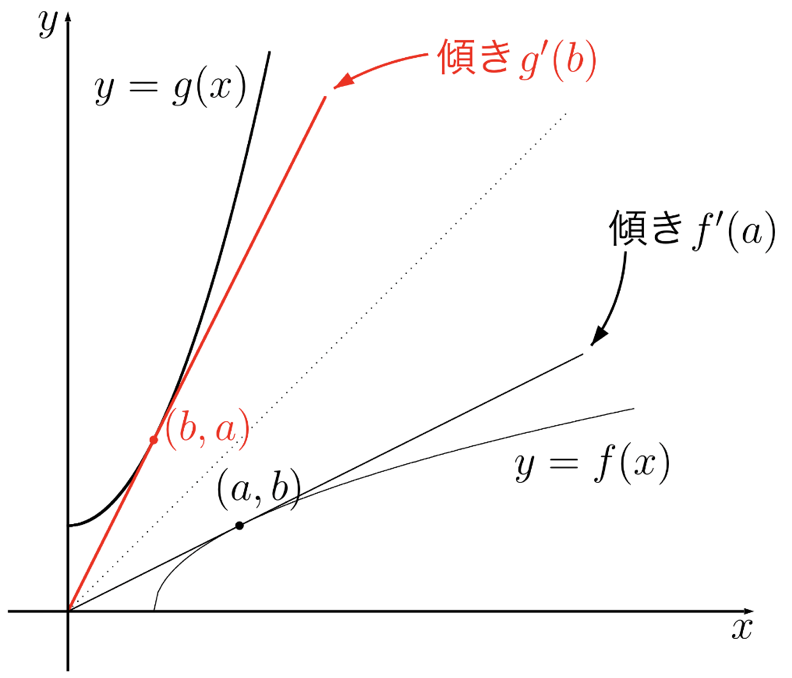
\includegraphics[width=65mm]{diff_inv.png}
 \end{center}
\end{figure}



\end{frame}



%%%%%%%%%%%%%%%%%%%%%%%%%%%%%%%%%%%%%%%%%%%%%%%%%%%%%%%%%%%%%%%%%%%%%%%%%%%%%%%%%%%%%%%
%%%%%%%%%%%%%%%%%%%%%%%%%%%%%%%%%%%%%%%%%%%%%%%%%%%%%%%%%%%%%%%%%%%%%%%%%%%%%%%%%%%%%%%


%\begin{frame}
%\frametitle{逆関数の微分}
%
%\begin{Prob}
%次の関数$f,g$は互いに逆関数の関係にあった. 
%\begin{enumerate}
%\item $f:\R \longrightarrow \R, \  x \mapsto 2x-4, \ \  g:\R \longrightarrow \R, \ y \mapsto \frac{1}{2}y+2$, 
%\item $f: \R \longrightarrow \R_+, \  x \mapsto e^x, \ \ g: \R_+ \longrightarrow \R, \ y \mapsto \log y$, 
%\item $f: \R_+ \longrightarrow \R_+,  \  x \mapsto x^2, \ \ g: \R_+ \longrightarrow \R_+,  \ y \mapsto \sqrt{y}$. 
%\end{enumerate}
%これらに関して, 逆関数の微分公式を確認せよ. 
%\end{Prob}
%
%\end{frame}



%%%%%%%%%%%%%%%%%%%%%%%%%%%%%%%%%%%%%%%%%%%%%%%%%%%%%%%%%%%%%%%%%%%%%%%%%%%%%%%%%%%%%%%
%%%%%%%%%%%%%%%%%%%%%%%%%%%%%%%%%%%%%%%%%%%%%%%%%%%%%%%%%%%%%%%%%%%%%%%%%%%%%%%%%%%%%%%


\begin{frame}
\frametitle{逆関数の微分}


関数
$$
f:\R \longrightarrow \R, \  x \mapsto 2x-4, \ \ \  g:\R \longrightarrow \R, \ y \mapsto \frac{1}{2}y+2
$$
は互いに逆写像の関係にあった. \\
\ \\

実際に導関数を計算してみると
$$
f'(x)=2, \ \ \ g'(y)= \frac{1}{2}
$$
であるから, 確かに
\begin{align*}
 \frac{1}{g'(2x-4)} = 2 = f'(x), \ \ \ \frac{1}{f'(\frac{1}{2}y+2)}=\frac{1}{2}=g'(y). 
\end{align*}



\end{frame}




%%%%%%%%%%%%%%%%%%%%%%%%%%%%%%%%%%%%%%%%%%%%%%%%%%%%%%%%%%%%%%%%%%%%%%%%%%%%%%%%%%%%%%%
%%%%%%%%%%%%%%%%%%%%%%%%%%%%%%%%%%%%%%%%%%%%%%%%%%%%%%%%%%%%%%%%%%%%%%%%%%%%%%%%%%%%%%%


\begin{frame}
\frametitle{逆関数の微分}


関数
\begin{align*}
f: \R \longrightarrow \R_+, \  x \mapsto e^x, \ \ \ 
g: \R_+ \longrightarrow \R, \ y \mapsto \log y
\end{align*}
は互いに逆写像の関係にあった. \\
\ \\

実際に導関数を計算してみると
$$
f'(x)=e^x, \ \ \ g'(y)= \frac{1}{y}
$$
であるから, 確かに
\begin{align*}
\frac{1}{g'(e^x)} = \frac{1}{\frac{1}{e^x}}=e^x, \ \ \ \frac{1}{f'(\log y)}=\frac{1}{e^{\log y}}=\frac{1}{y}=g'(y). 
\end{align*}



\end{frame}



%%%%%%%%%%%%%%%%%%%%%%%%%%%%%%%%%%%%%%%%%%%%%%%%%%%%%%%%%%%%%%%%%%%%%%%%%%%%%%%%%%%%%%%
%%%%%%%%%%%%%%%%%%%%%%%%%%%%%%%%%%%%%%%%%%%%%%%%%%%%%%%%%%%%%%%%%%%%%%%%%%%%%%%%%%%%%%%


\begin{frame}
\frametitle{逆関数の微分}


関数
\begin{align*}
f: \R_+ \longrightarrow \R_+,  \  x \mapsto x^2, \ \ \ g: \R_+ \longrightarrow \R_+,  \ y \mapsto \sqrt{y}
\end{align*}
は互いに逆写像の関係にあった. \\
\ \\

実際に導関数を計算してみると
$$
f'(x)=2x, \ \ \ g'(y)= \frac{1}{2\sqrt{y}}
$$
であるから, 確かに
\begin{align*}
 \frac{1}{g'(x^2)} = \frac{1}{\frac{1}{2\sqrt{x^2}}}=2x =f'(x), \ \ \ \frac{1}{f'(\sqrt{y})}=\frac{1}{2\sqrt{y}}=g'(y). 
\end{align*}



\end{frame}



%%%%%%%%%%%%%%%%%%%%%%%%%%%%%%%%%%%%%%%%%%%%%%%%%%%%%%%%%%%%%%%%%%%%%%%%%%%%%%%%%%%%%%%
%%%%%%%%%%%%%%%%%%%%%%%%%%%%%%%%%%%%%%%%%%%%%%%%%%%%%%%%%%%%%%%%%%%%%%%%%%%%%%%%%%%%%%%


\begin{frame}
\frametitle{逆関数の微分}

\begin{Prob}
$f(x)=\sqrt[3]{x}$の逆関数を求め, 逆関数の微分法(定理\ref{逆関数の微分定理})が成立していることを確かめよ. 
\end{Prob}

\end{frame}



%%%%%%%%%%%%%%%%%%%%%%%%%%%%%%%%%%%%%%%%%%%%%%%%%%%%%%%%%%%%%%%%%%%%%%%%%%%%%%%%%%%%%%%
%%%%%%%%%%%%%%%%%%%%%%%%%%%%%%%%%%%%%%%%%%%%%%%%%%%%%%%%%%%%%%%%%%%%%%%%%%%%%%%%%%%%%%%


\begin{frame}
\frametitle{逆関数の微分}


$f(x)=\sqrt[3]{x}$の逆関数は$g(y)=y^3$である. 導関数はそれぞれ
$$
f'(x)=\frac{1}{3 \sqrt[3]{x^2}}, \ \ \ g'(y)=3y^2
$$
であるから, 確かに
$$
\frac{1}{g'(\sqrt[3]{x})}=\frac{1}{3\sqrt[3]{x}^2}=f'(x), \ \ \ 
\frac{1}{f'(y^3)}=\frac{1}{\frac{1}{3 \sqrt[3]{(y^3)^2}}}=g'(y). 
$$

\end{frame}



%%%%%%%%%%%%%%%%%%%%%%%%%%%%%%%%%%%%%%%%%%%%%%%%%%%%%%%%%%%%%%%%%%%%%%%%%%%%%%%%%%%%%%%
%%%%%%%%%%%%%%%%%%%%%%%%%%%%%%%%%%%%%%%%%%%%%%%%%%%%%%%%%%%%%%%%%%%%%%%%%%%%%%%%%%%%%%%


%\begin{frame}
%\frametitle{逆関数の微分}
%
%
%$f_2(x)=x^2+4x-1$の逆関数は, $x^2+4x-1-y=0$を$x$について解いて
%$$
%g_2(y)=-2 \pm \sqrt{y+5}. 
%$$
%導関数はそれぞれ
%$$
%f_2'(x)=2x+4, \ \ \ g_2'(y)=\pm \frac{1}{2\sqrt{y+5}}
%$$
%であるから, 確かに
%\begin{align*}
%\frac{1}{g_2'(x^2+4x-1)} &= \frac{1}{\pm \frac{1}{2\sqrt{x^2+4x-1+5}}} =\pm 2(x+2)=\\
%\frac{1}{f_2'(-2 \pm \sqrt{y+5})} & = \frac{1}{2(-2 \pm \sqrt{y+5})+4}=g_2'(y). 
%\end{align*}
%
%\end{frame}



%%%%%%%%%%%%%%%%%%%%%%%%%%%%%%%%%%%%%%%%%%%%%%%%%%%%%%%%%%%%%%%%%%%%%%%%%%%%%%%%%%%%%%%
%%%%%%%%%%%%%%%%%%%%%%%%%%%%%%%%%%%%%%%%%%%%%%%%%%%%%%%%%%%%%%%%%%%%%%%%%%%%%%%%%%%%%%%

\section{逆三角関数}

\begin{frame}
\frametitle{三角関数}

三角関数$\sin x, \cos x, \tan x$を思い出す. 


 \begin{figure}[htbp]
 \begin{center} 
  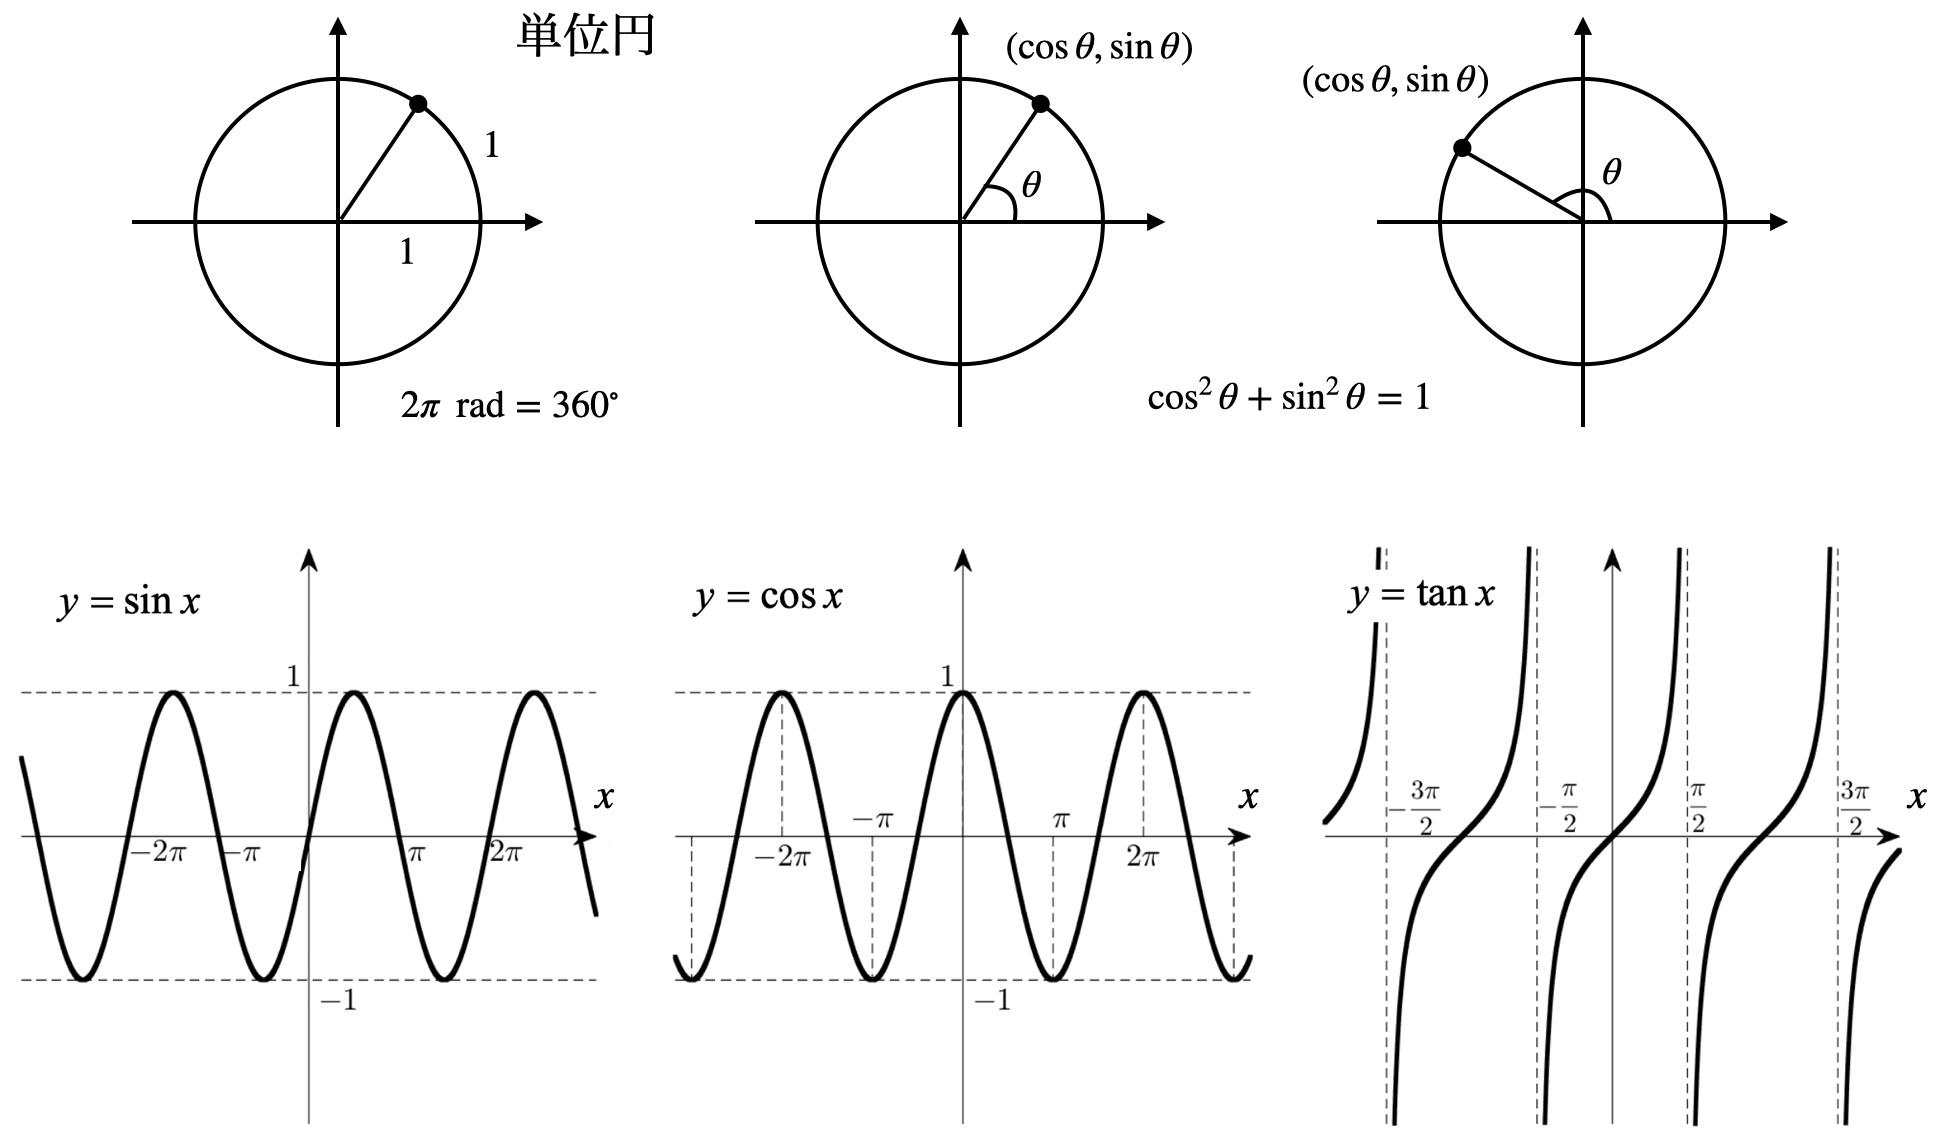
\includegraphics[width=100mm]{trig2.png}
 \end{center}
\end{figure}


\end{frame}



%%%%%%%%%%%%%%%%%%%%%%%%%%%%%%%%%%%%%%%%%%%%%%%%%%%%%%%%%%%%%%%%%%%%%%%%%%%%%%%%%%%%%%%
%%%%%%%%%%%%%%%%%%%%%%%%%%%%%%%%%%%%%%%%%%%%%%%%%%%%%%%%%%%%%%%%%%%%%%%%%%%%%%%%%%%%%%%


\begin{frame}
\frametitle{逆三角関数}

\begin{itemize}
\item $\sin:[-\pi/2,\pi/2]\rightarrow [-1,1]$は全単射. 
この逆関数を$\arcsin x$と書く. 
$$
\arcsin: [-1,1] \longrightarrow [-\pi/2,\pi/2], \ \ \ x \mapsto \arcsin x. 
$$
\item $\cos:[0,\pi]\rightarrow [-1,1]$は全単射. 
この逆関数を$\arccos x$と書く. 
$$
\arccos: [-1,1] \longrightarrow [0,\pi], \ \ \ x \mapsto \arccos x. 
$$
\item $\tan:(-\pi/2,\pi/2)\rightarrow \R$は全単射. 
この逆関数を$\arctan x$と書く. 
$$
\arctan: \R \longrightarrow (-\pi/2,\pi/2), \ \ \ x \mapsto \arctan x. 
$$
\end{itemize}
これらは逆三角関数と呼ばれ, それぞれ$\sin^{-1}x, \cos^{-1}x,\tan^{-1}x$と書くこともある. 
($\arcsin x = \sin^{-1}x \neq \frac{1}{\sin x}$)




\end{frame}



%%%%%%%%%%%%%%%%%%%%%%%%%%%%%%%%%%%%%%%%%%%%%%%%%%%%%%%%%%%%%%%%%%%%%%%%%%%%%%%%%%%%%%%
%%%%%%%%%%%%%%%%%%%%%%%%%%%%%%%%%%%%%%%%%%%%%%%%%%%%%%%%%%%%%%%%%%%%%%%%%%%%%%%%%%%%%%%


\begin{frame}
\frametitle{逆三角関数}



 \begin{figure}[htbp]
 \begin{center} 
  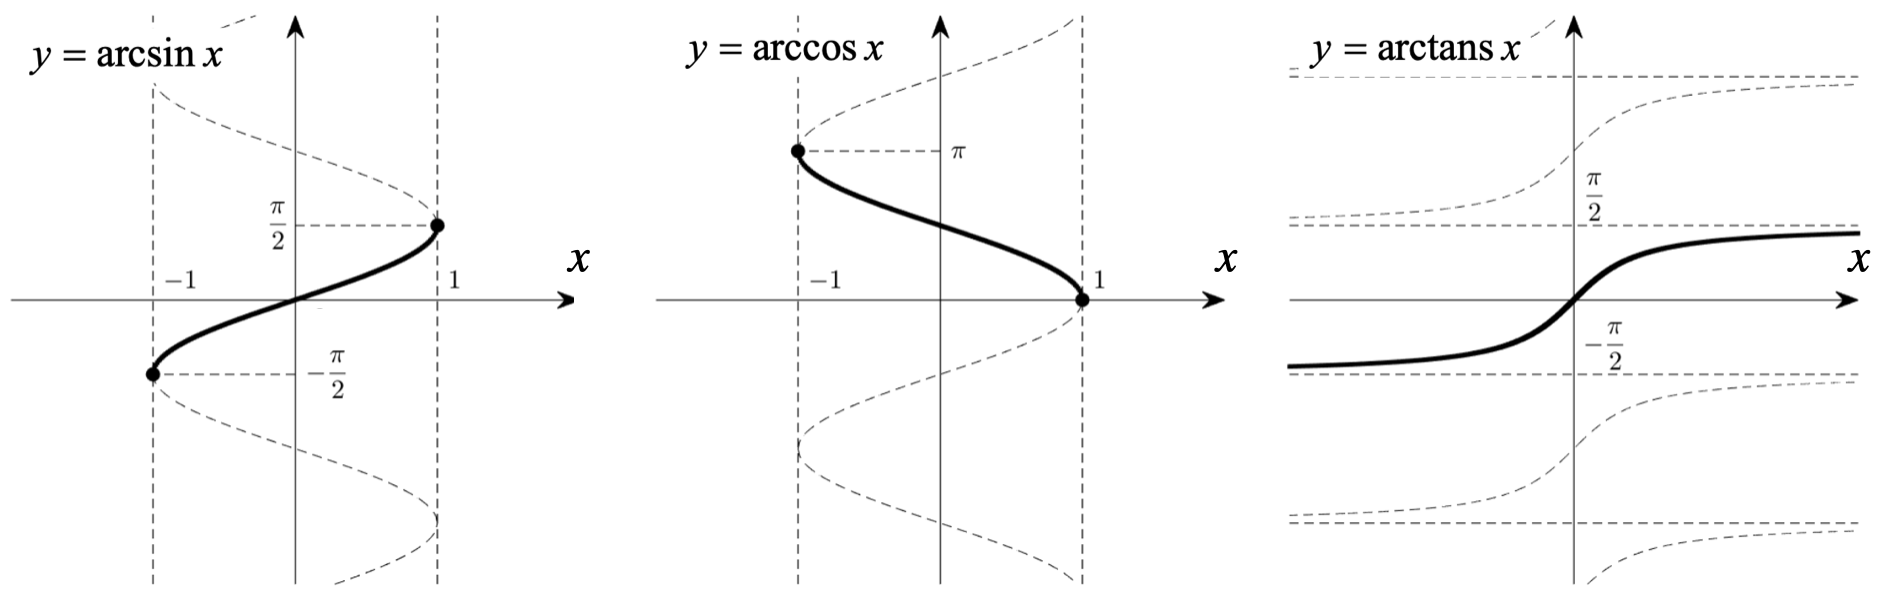
\includegraphics[width=120mm]{inv_trig.png}
 \end{center}
\end{figure}


\end{frame}


%%%%%%%%%%%%%%%%%%%%%%%%%%%%%%%%%%%%%%%%%%%%%%%%%%%%%%%%%%%%%%%%%%%%%%%%%%%%%%%%%%%%%%%
%%%%%%%%%%%%%%%%%%%%%%%%%%%%%%%%%%%%%%%%%%%%%%%%%%%%%%%%%%%%%%%%%%%%%%%%%%%%%%%%%%%%%%%


\begin{frame}
\frametitle{逆三角関数}

%実際, $0 \le x \le 1$に関して, 逆関数は$\arcsin x$と$\arccos x$は半径$\frac{1}{2}$の円の弧(arc)の一部の長さを表している. 
実際, $0 \le x \le 1$に関して, $\arcsin x$と$\arccos x$は半径$1$の円の弧(arc)の一部の長さを表している. 

 \begin{figure}[htbp]
 \begin{center} 
  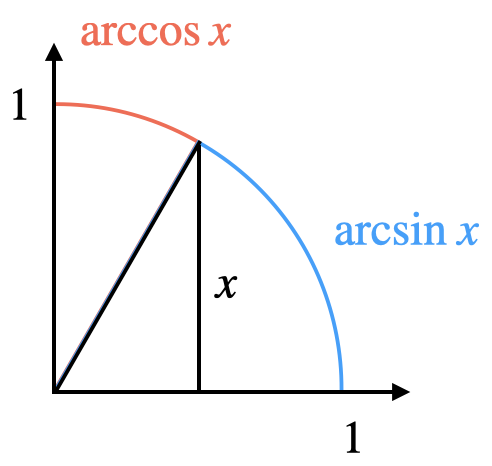
\includegraphics[width=38mm]{arc2.png}
 \end{center}
\end{figure}
\vspace{-3mm}

これより, 例えば
$$
\arcsin x + \arccos x = \frac{\pi}{2}
$$
が視覚的に理解できる. ($-1\le x \le 1$で成立.)

\end{frame}


%%%%%%%%%%%%%%%%%%%%%%%%%%%%%%%%%%%%%%%%%%%%%%%%%%%%%%%%%%%%%%%%%%%%%%%%%%%%%%%%%%%%%%%
%%%%%%%%%%%%%%%%%%%%%%%%%%%%%%%%%%%%%%%%%%%%%%%%%%%%%%%%%%%%%%%%%%%%%%%%%%%%%%%%%%%%%%%


\begin{frame}
\frametitle{逆三角関数}



\begin{Prob}
次の値を求めよ. 
\begin{enumerate}
\item $\arcsin \frac{1}{\sqrt{2}}$,  %\pi/4
\item $\arcsin 1$, %\pi/2
\item $\arccos \frac{1}{2}$, %\pi/3 
\item $\arctan \frac{1}{\sqrt{3}}$ % \pi/6
\end{enumerate}
\end{Prob}

\end{frame}



%%%%%%%%%%%%%%%%%%%%%%%%%%%%%%%%%%%%%%%%%%%%%%%%%%%%%%%%%%%%%%%%%%%%%%%%%%%%%%%%%%%%%%%
%%%%%%%%%%%%%%%%%%%%%%%%%%%%%%%%%%%%%%%%%%%%%%%%%%%%%%%%%%%%%%%%%%%%%%%%%%%%%%%%%%%%%%%


\section{逆三角関数の微分}

\begin{frame}
\frametitle{逆三角関数}

\begin{Thm}
$$
(\arcsin x)'=\frac{1}{\sqrt{1-x^2}}
$$
\end{Thm}

$f(x)=\arcsin x$の逆関数は$g(y)=\sin y$であるから
\begin{align*}
f'(x)=\frac{1}{g'(y)}=\frac{1}{\cos y}=\frac{1}{\sqrt{1-x^2}}. 
\end{align*}
ただし最後に
$$
\cos y = \sqrt{1-\sin^2 y}=\sqrt{1-x^2}
$$
を用いた. 


\end{frame}



%%%%%%%%%%%%%%%%%%%%%%%%%%%%%%%%%%%%%%%%%%%%%%%%%%%%%%%%%%%%%%%%%%%%%%%%%%%%%%%%%%%%%%%
%%%%%%%%%%%%%%%%%%%%%%%%%%%%%%%%%%%%%%%%%%%%%%%%%%%%%%%%%%%%%%%%%%%%%%%%%%%%%%%%%%%%%%%


\begin{frame}
\frametitle{逆三角関数}

\begin{Thm}
$$
(\arccos x)'= - \frac{1}{\sqrt{1-x^2}}
$$
\end{Thm}

$f(x)=\arccos x$の逆関数は$g(y)=\cos y$であるから
\begin{align*}
f'(x)=\frac{1}{g'(y)}=\frac{1}{- \sin y}=-\frac{1}{\sqrt{1-x^2}}. 
\end{align*}
\end{frame}


%%%%%%%%%%%%%%%%%%%%%%%%%%%%%%%%%%%%%%%%%%%%%%%%%%%%%%%%%%%%%%%%%%%%%%%%%%%%%%%%%%%%%%%
%%%%%%%%%%%%%%%%%%%%%%%%%%%%%%%%%%%%%%%%%%%%%%%%%%%%%%%%%%%%%%%%%%%%%%%%%%%%%%%%%%%%%%%


\begin{frame}
\frametitle{逆三角関数}

\begin{Thm}
$$
(\arctan x)'= \frac{1}{1+x^2}
$$
\end{Thm}

$f(x)=\arctan x$の逆関数は$g(y)=\tan y$であるから
\begin{align*}
f'(x)=\frac{1}{g'(y)}=\frac{1}{\frac{1}{\cos^2 y}}=\cos^2 y = \frac{1}{1+x^2}.  
\end{align*}
ただし最後に
$$
\cos^2 y \cdot (1+\tan^2 y)=\cos^2 y + \sin^2 y = 1
$$
を用いた. 

\end{frame}


%%%%%%%%%%%%%%%%%%%%%%%%%%%%%%%%%%%%%%%%%%%%%%%%%%%%%%%%%%%%%%%%%%%%%%%%%%%%%%%%%%%%%%%
%%%%%%%%%%%%%%%%%%%%%%%%%%%%%%%%%%%%%%%%%%%%%%%%%%%%%%%%%%%%%%%%%%%%%%%%%%%%%%%%%%%%%%%


\begin{frame}
\frametitle{逆三角関数}

\begin{Prob}
次の関数の導関数を求めよ. 
\begin{enumerate}
\item $\arcsin 3x^2$, 
\item $\arctan (x^3+1)$
\end{enumerate}
\end{Prob}

\end{frame}

%%%%%%%%%%%%%%%%%%%%%%%%%%%%%%%%%%%%%%%%%%%%%%%%%%%%%%%%%%%%%%%%%%%%%%%%%%%%%%%%%%%%%%%
%%%%%%%%%%%%%%%%%%%%%%%%%%%%%%%%%%%%%%%%%%%%%%%%%%%%%%%%%%%%%%%%%%%%%%%%%%%%%%%%%%%%%%%





%%%%%%%%%%%%%%%%%%%%%%%%%%%%%%%%%%%%%%%%%%%%%%%%%%%%%%%%%%%%%%%%%%%%%%%%%%%%%%%%%%%%%%%
%%%%%%%%%%%%%%%%%%%%%%%%%%%%%%%%%%%%%%%%%%%%%%%%%%%%%%%%%%%%%%%%%%%%%%%%%%%%%%%%%%%%%%%




\section{今日のまとめ}
\begin{frame}
\frametitle{まとめ}   

\begin{enumerate}
\item 逆写像, 逆関数, 逆関数の微分
\item 逆三角関数, 逆三角関数の微分
\end{enumerate} 




\end{frame}


\end{document}